\documentclass[../notes.tex]{subfiles}

\pagestyle{main}
\renewcommand{\chaptermark}[1]{\markboth{\chaptername\ \thechapter\ (#1)}{}}
\setcounter{chapter}{3}

\begin{document}




\chapter{Electronic and Magnetic Spectroscopy}
\section{Lecture 7: Electronic Molecular Spectroscopy}
\begin{itemize}
    \item \marginnote{1/24:}Lant check in on lab.
    \begin{itemize}
        \item The clean up process is still going on; we're not getting back in the lab for the rest of the quarter. We'll still meet in Jones 108, but not use the PChem lab.
        \item When cleaning up the small barometer spill, they found a much larger spill covered in dust that's been there for who knows how many years, so they're having to bring in a professional team and it will take weeks. They don't just have to get it down to OSHA levels; it's an educational environment, so the requirements are even more stringent.
        \item They may or may not be able to still offer every lab.
        \item Lant is open to questions.
        \item Most of us should be totally fine.
        \item They found a line of it behind the hood.
    \end{itemize}
    \item Announcements.
    \begin{itemize}
        \item No lecture on Thursday; OH then in Searle 240.
        \item NMR lecture next week.
        \item Detailed guidelines on the long report by the end of the week.
    \end{itemize}
    \item Today: Electronic spectroscopy and the \ce{I2} absorption data.
    \item This is electronic \emph{molecular} spectroscopy where electrons are localized, in contrast to electronic \emph{nanomaterial} spectroscopy for example.
    \item We focus on valence electrons.
    \begin{itemize}
        \item These absorb UV/Vis light.
        \item Light absorption changes electronic charge distribution around the molecule; a lot of energy allows you to break bonds.
        \item Molecules change all states, but start in the electronic ground state.
        \item We will not look at core electrons here; we'd need X-rays for that. This is atom specific.
    \end{itemize}
    \item Types of molecular electronic transitions.
    \begin{itemize}
        \item In organic compounds, we're usually looking at $\sigma\to\sigma^*$ or $\pi\to\pi^*$ transitions, typically in unsaturated compounds.
        \item In saturated compounds, it is extremely difficult to get excitations, and we have to go into the deep UV.
    \end{itemize}
    \item Example: Coumarin 153 dye.
    \begin{itemize}
        \item Which HOMO and LUMO change, as well as the net change in dipole.
    \end{itemize}
    \item Inorganic spectroscopy.
    \begin{itemize}
        \item $d\to d$ and charge transfer; related to \ce{Ru(bpy)3^2+}.
    \end{itemize}
    \item Electronic spectra of diatomic molecules.
    \begin{itemize}
        \item Lots of fine structure: Primarily changes in vibrational quantum number.
        \item The rotational constant of massive \ce{I2} is very small; thus, we just can't resolve it here.
    \end{itemize}
    \item Electronic spectra of diatomic molecules.
    \emph{picture}
    \begin{itemize}
        \item Transition to higher energy across potential energy surfaces.
        \item \textbf{Bound} vs. \textbf{dissociative} surfaces.
        \item \textbf{Franck-Condon principle}: The big one for electronic spectroscopy. Along the same lines as the BO approximation, we assume that electronic configuration can change/be excited much more quickly than the nuclei can move, so we fix the nuclei when we study electronic changes. Corresponds to \emph{vertical} transitions.
        \item Electronic excitation results in unstable configuration. More force on the atom as it tries to lengthen its bond causes it to vibrate more.
    \end{itemize}
    \item Potential energy surfaces of \ce{I2}.
    \begin{itemize}
        \item We get a transition from the X to the B state that increases bond length.
        \item \ce{I2} is a massively anharmonic oscillator (hard repulsive wall; softer attractive wall).
        \item Vibrational spacing $\Delta v$ decreases with increasing energy.
        \item Different shaped potentials (different bond lengths and different vibrational splittings).
    \end{itemize}
    \item UV/Vis spectroscopy of \ce{I2}.
    \begin{figure}[h!]
        \centering
        \begin{subfigure}[b]{0.49\linewidth}
            \centering
            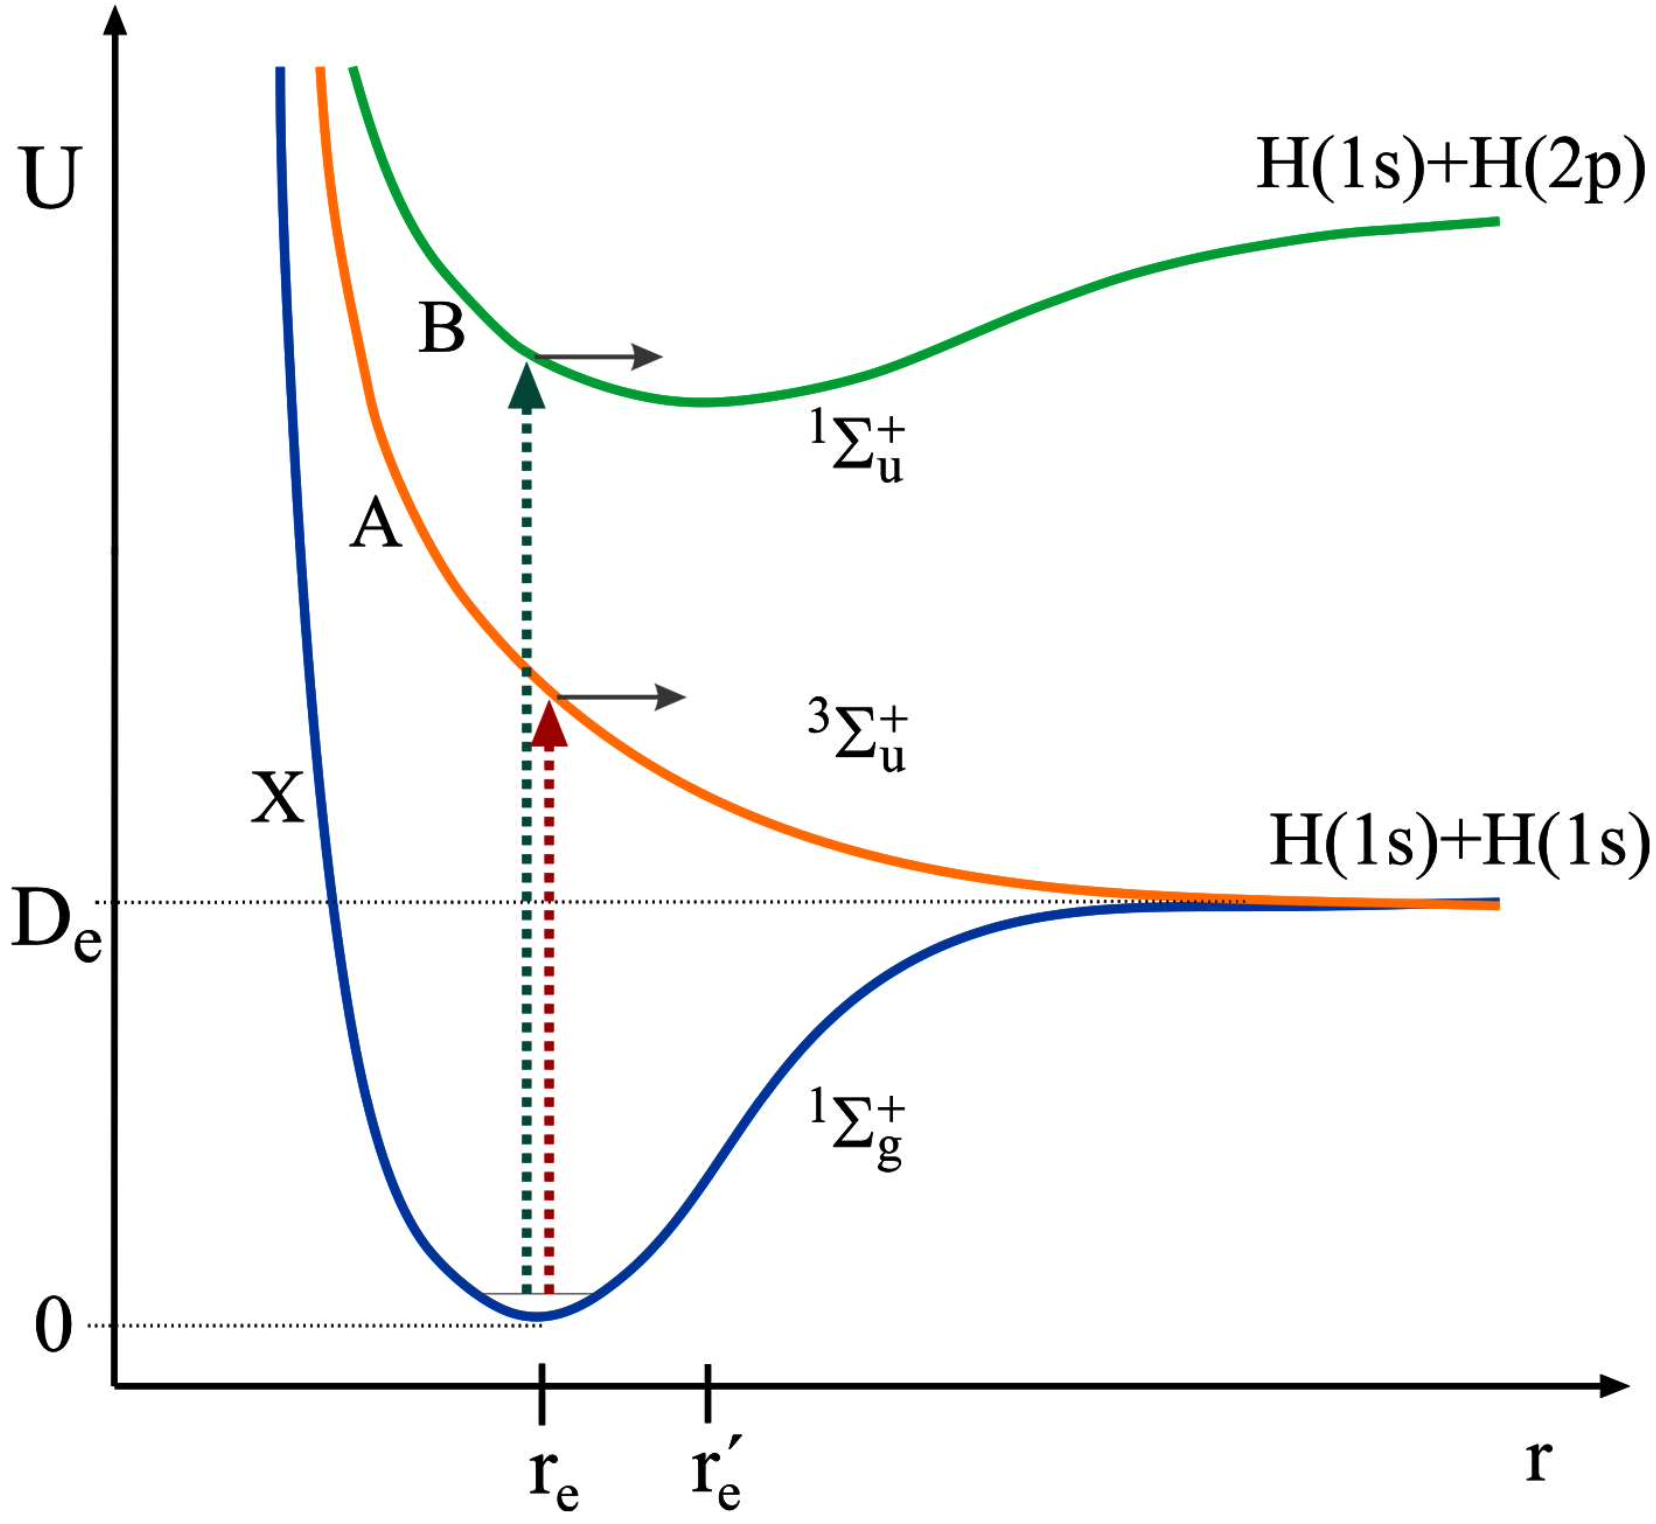
\includegraphics[width=0.8\linewidth]{FCFa.png}
            \caption{Vibrational excitation.}
            \label{fig:FCFa}
        \end{subfigure}
        \begin{subfigure}[b]{0.49\linewidth}
            \centering
            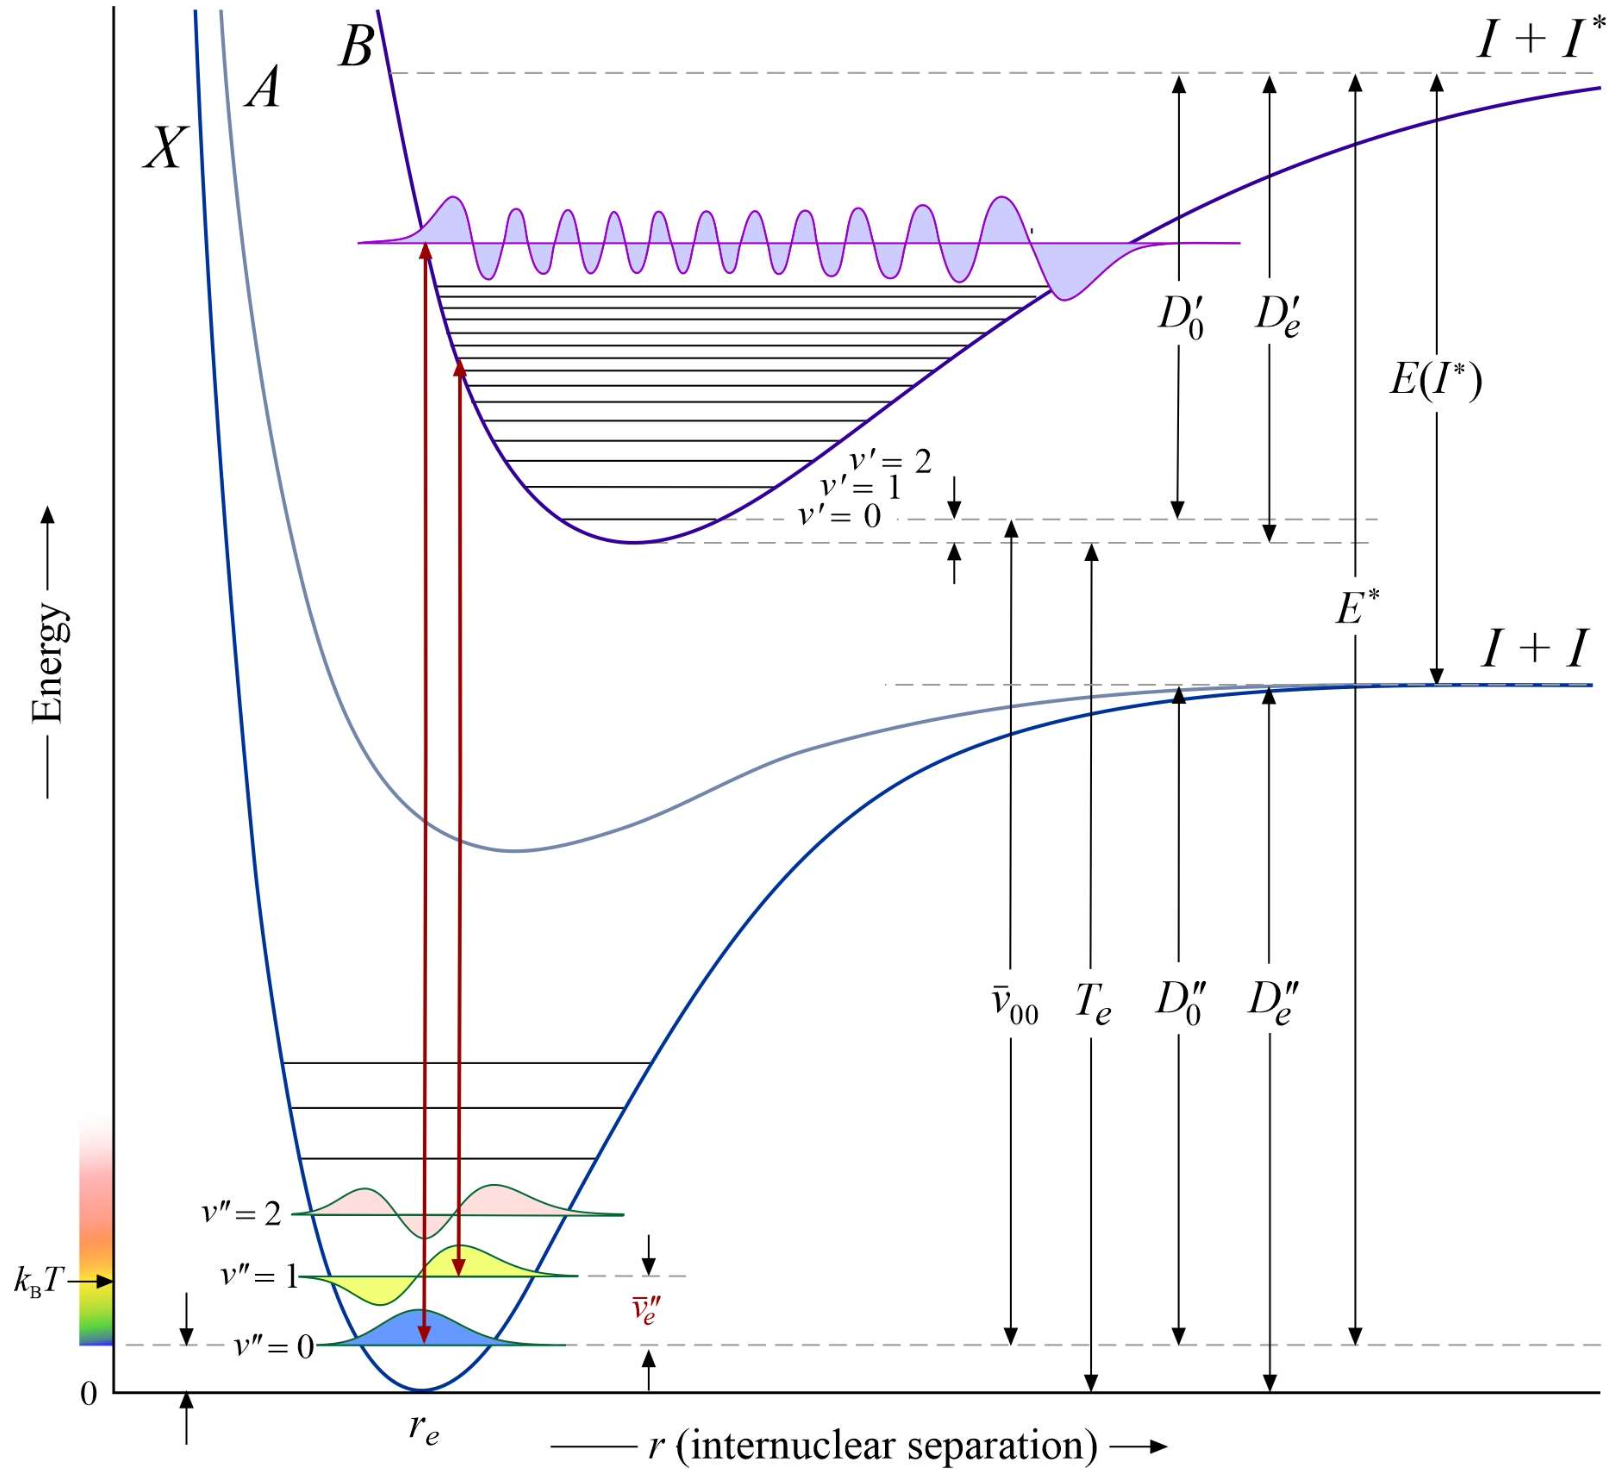
\includegraphics[width=0.8\linewidth]{FCFb.png}
            \caption{Wavefunction overlap.}
            \label{fig:FCFb}
        \end{subfigure}
        \caption{Franck-Condon factors in electronic spectroscopy.}
        \label{fig:FCF}
    \end{figure}
    \begin{itemize}
        \item Franck-Condon implies a vertical transition; this implies significant vibrational excitation since vertically above the equilibrium is an excited vibrational state.
        \begin{itemize}
            \item In particular, we get excitation to the classical turning point.
        \end{itemize}
        \item We need good overlap between vibrational wavefunctions to get excitation (also by Franck-Condon).
        \item There are resonances with many states, especially since higher-energy vibrational states are so tightly spaced. This is what gives vibrational fine structure.
        \item The transition spacing converges on the dissociation energy. From the 0-0 transition ($v''=v'=0$) and convergence limit, we can get $D_0'$.
        \item Low frequency vibration of the X state implies that $v''=1,2$ will be thermally occupied as well. This allows access to lower vibrational excited states because this wavefunction extends farther and can overlap with lower.
        \item There is also an excited A state between the X and the B state.
        \item To measure $v''=0$ transitions all the way down, you need to eliminate the hot bands. To do this, cool your sample down to a few degrees kelvin (reduces thermal occupation of higher states).
    \end{itemize}
    \item Reconstructing a potential from absorption spectra.
    \begin{itemize}
        \item Can't resolve rotational transitions.
        \begin{itemize}
            \item The sawtooth structure hides the rotational transitions.
        \end{itemize}
        \item Assign transitions.
        \item Use spacing to get information.
        \item The frequency of the transition is related to the bare electronic transition, plus vibrational fine structure.
    \end{itemize}
    \item Tons of good stuff on UV-Vis that may be worth rewatching at some point!!!
    \item Isolate X and B state frequencies.
    \begin{itemize}
        \item Changes in $v'$ vs. $v''$.
        \item You can go from frequencies to dissociation constants with additional equations.
    \end{itemize}
    \item \textbf{Birge-Sponer plot}: A plot of the vibrational frequency vs. the final vibrational quantum number.
    \begin{itemize}
        \item At higher and higher vibrational quantum numbers, we get closer to the dissociation threshold and see deviation from linearity.
        \item If it deviates to higher vibrational quantum numbers, the potential is a bit softer; otherwise, it's a bit steeper.
        \item The $y$-intercept also tells you the maximum transition you can get to before dissociating.
    \end{itemize}
    \item Selection rules for electronic spectroscopy.
    \begin{itemize}
        \item \emph{We} won't have to analyze intensity, but it does convey a lot of important information.
        \item Absorption requires that resonance creates changes in electronic charge density, i.e.,
        \begin{equation*}
            \pdv{\mu}{q} \neq 0
        \end{equation*}
        \begin{itemize}
            \item Technically, we need a change in parity/inversion from $u\leftrightarrow g$.
        \end{itemize}
        \item Transition probability involves nuclear and electronic degrees of freedom.
        \item Vibrational wave functions are on different electronic surfaces.
        \item Related to both the electronic transition dipole moment and the Franck-Condon overlap integral.
        \item Thus, the maximum intensity tells us about the displacement between $r_e''$ and $r_e'$.
        \item Franck-Condon factors (FCF's) for harmonic oscillators are discussed.
        \item We can talk to Tokmakoff about this if we \emph{want} to do it in our report.
    \end{itemize}
    \item After absorption.
    \begin{itemize}
        \item A word on fluorescence (useful for later experiments).
        \item Energy has to dissipate to return to equilibrium.
        \item Options.
        \begin{itemize}
            \item Energy transfer and relaxation processes (within and between molecules).
            \item Electron transfer.
            \item Photochemistry.
            \item Radiative relaxation.
        \end{itemize}
        \item High probability/fast processe dominate.
    \end{itemize}
    \item Relaxation of electronic states.
    \begin{figure}[h!]
        \centering
        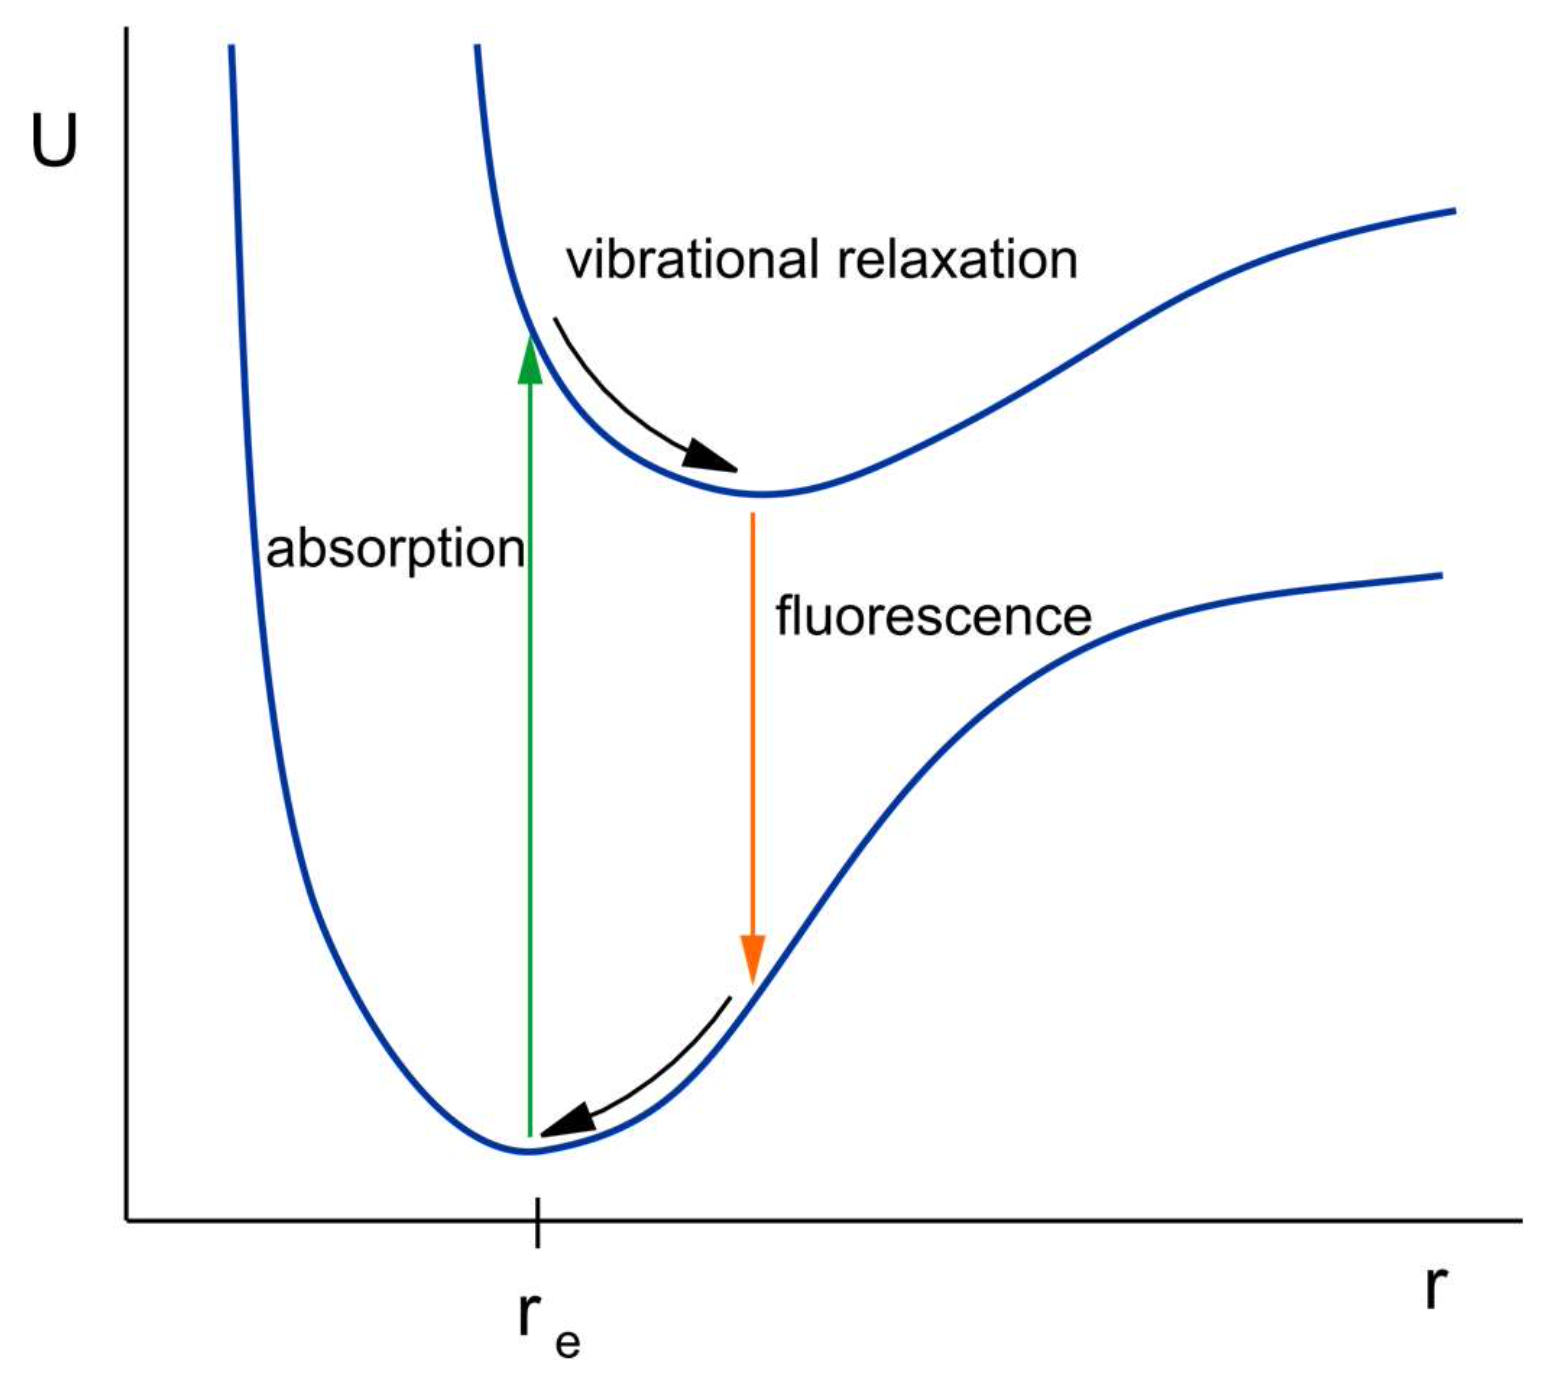
\includegraphics[width=0.4\linewidth]{fluorescence.png}
        \caption{UV/Vis fluorescence.}
        \label{fig:fluorescence}
    \end{figure}
    \begin{itemize}
        \item We get a displacement of charge and a new equilibrium nuclear separation.
        \item More vibrational energy is dissipated nonradiatively.
        \item A huge amount of energy is released to the ground state, typically through flourescence.
        \item Naturally, fluorescence is always red-shifted relative to absorption.
        \item We call the red shift the \textbf{Stokes shift} and denote it by $2\lambda$.
    \end{itemize}
\end{itemize}



\section{Lecture 8: Magnetic Resonance Spectroscopy}
\begin{itemize}
    \item \marginnote{1/26:}Refer to Chapter 14 of \textcite{bib:McQuarrieSimon}.
    \item There is both NMR (nuclear magnetic resonance) and ESR (electron spin resonance) or EPR (electron paramagnetic resonance).
    \begin{itemize}
        \item The last two are the same thing.
    \end{itemize}
    \item Two fields: The static magnetic field, and the probing \emph{electro}magnetic field.
    \item Derivation of quantized angular momentum.
    \begin{itemize}
        \item In molecules, there is a multiplicity/degeneracy of states that grows as $2J+1$. They have quantized angular momentum.
        \item So is the orbital angular momentum of electrons!
        \item Putting atoms into a magnetic field \emph{creates} the anisotropy necessary for discussing the $z$-component (or any coordinate component) of angular momentum.
        \item Spin angular momentum: Just means that the objects (e.g., electrons and nuclei) have a property that looks a lot like spin and/or angular momentum.
        \item We say that each nucleon has a spin of $1/2$. Protons and neutrons add separately.
        \begin{itemize}
            \item Even number of protons and neutrons? Spin 0.
            \item Mixed even/odd? We have actual nuclear spin.
            \begin{itemize}
                \item We need a nucleus like this to detect!
            \end{itemize}
            \item Odd/odd? We have 0 spin again.
        \end{itemize}
        \item We focus on spin $1/2$ particles. These have two degenerate energy states that split in a magnetic field.
    \end{itemize}
    \item Classical picture of spin angular momentum.
    \begin{itemize}
        \item Picture a charged particle with angular momentum. The circulating charge produced a magnetic field which aligns along the direction of the angular momentum.
        \item Indeed, a spinning charged particle behaves like a dipole.
        \item $\gamma=2mc$ is the \textbf{gyromagnetic ratio}.
    \end{itemize}
    \item Quantum spin angular momentum.
    \begin{itemize}
        \item Basically the same thing; we just rephrase everything from before in the language of operators.
    \end{itemize}
    \item \textbf{Zeeman effect}: Two energy levels split with increasing $B$.
    \item \textbf{Larmor frequency}: The frequency $\nu=\gamma B/2\pi$ in the radio frequency range that induces a shift.
    \item Typical operating conditions.
    \begin{itemize}
        \item NMR vs. ESR: NMR has a stronger magnetic field, longer EM excitation radio waves, and significantly lower gyromagnetic ratios.
        \item There is only a tiny difference between nuclear state occupation at room temperature; hence supercooling to get something detectable.
    \end{itemize}
    \item What is the magnetic dipole doing in the magnetic field?
    \begin{itemize}
        \item No constraints on the $x$ and $y$ components of $I$.
        \item A dipole in a field experiences a torque.
        \begin{itemize}
            \item Dipole precesses around $B$ at the Larmor frequency $\nu$.
        \end{itemize}
        \item FT-NMR spectrometers use pulsed rf fields to synchronize and detect the procession of spins.
    \end{itemize}
    \item Lots of good extension material on NMR; also worth rewatching at some point!
\end{itemize}




\end{document}